\documentclass[]{exam}

\usepackage{verbatim, multicol, tabularx,hyperref, tikz, tikz-qtree, enumitem}
\usepackage{amsmath,amsthm, amssymb, stmaryrd, latexsym, bm, listings}
\usepackage[margin=1in]{geometry}

\lstset{
  extendedchars=\true,
  inputencoding=utf8,
  literate=
  {é}{{\'{e}}}1
  {è}{{\`{e}}}1
  {ê}{{\^{e}}}1
  {ë}{{\¨{e}}}1
  {û}{{\^{u}}}1
  {ù}{{\`{u}}}1
  {â}{{\^{a}}}1
  {à}{{\`{a}}}1
  {î}{{\^{i}}}1
  {ô}{{\^{o}}}1
  {ç}{{\c{c}}}1
  {Ç}{{\c{C}}}1
  {É}{{\'{E}}}1
  {Ê}{{\^{E}}}1
  {À}{{\`{A}}}1
  {Â}{{\^{A}}}1
  {Î}{{\^{I}}}1
  {Ö}{{\"O}}1
  {Ä}{{\"A}}1
  {Ü}{{\"U}}1
  {ö}{{\"o}}1
  {ä}{{\"a}}1
  {ü}{{\"u}}1
  {ß}{{\ss}}1
  ,
  aboveskip=1mm,
  belowskip=1mm,
  showstringspaces=false,
  columns=flexible,
  basicstyle={\scriptsize\ttfamily},
  numbers=left,
  frame=single,
  framextopmargin=0pt,
  framexbottommargin=0pt,
  breaklines=true,
  breakatwhitespace=true,
  keywordstyle=\color{blue},
  identifierstyle=\color{violet},
  stringstyle=\color{teal},
  commentstyle=\color{darkgray}
}

\hypersetup{colorlinks=true,urlcolor=blue}

\headheight = 0.05 in
\headsep = 0.05 in
\parskip = 0.05in
\parindent = 0.0in
\floatsep = 0.05in

\DeclareMathOperator*{\argmin}{arg\!min}
\DeclareMathOperator*{\argmax}{arg\!max}

\title{Problem Solving Review}
\author{Artificial Intelligence}
\date{}

\begin{document}
\maketitle

\begin{questions}


\setcounter{section}{0} % So that next \section is 1

\question What is a planning problem?

\begin{solution}[1in]
A problem whose solutions are sequences of actions from some initial or current state to a goal state.
\end{solution}

\question Describe open-loop and closed-loop control.

\begin{solution}[1.5in]
In an open-loop control system the agent gets no feedback, i.e., sensor input, after executing an action.  If the agent's model is perfect and actions are deterministic, then the agent can operate in an open-loop fashion, simply executing the actions in the solution one after the other.

In a closed-loop control system the agent gets sensory feedback after every action, so it can check whether the action had the expected effect.  If the environment is partially observable or actions are nondeterministic, closed-loop control is necessary.

\end{solution}

\question Write a problem formulation for a world with three unmarked pitchers -- an 8 L pitcher full of water, an empty 5 L pitcher, and an empty 3 L pitcher -- where an agent must reallocate the water so that one of the pitchers contains exactly 4 L of water.

\begin{solution}[1in]
One of many possibilities:
\begin{itemize}
\item States: $\bm{p} = <p_1, p_2, p_3>$, $p_i \in \mathbb{N}$,  $\sum_{i = 1}^3 p_i = 8$,  $c_1 = 8, c_2 = 5, c_3 = 3$, $r_i = c_i - p_i$
\item Initial state:$<8, 0, 0>$
\item Actions: $Actions(\bm{p}) = pour(f, t)$ for all $f, t$ where $f, t \in {1,2,3}$ and $f \ne t$ and $p_f > 0$ and $r_t > 0$.  Examples:

\begin{itemize}
\item $actions(<8, 0, 0>) = \{pour(1, 2), pour(1, 3)\}$
\item $actions(<3, 5, 0>) = \{pour(1, 3), pour(2, 1), pour(2, 3)\}$
\end{itemize}

\item Transition model:

$$
RESULT(pour(f, t)) =
\begin{cases}
p_t \gets c_t, p_f \gets p_f -  r_t &\text{if } r_t \le p_f \\
p_t \gets p_t + p_f, p_f \gets 0 &\text{if } r_t \ge p_f
\end{cases}
$$

\item Goal states: $p_i = 4$ for some $i \in \{1, 2, 3\}$
\item Action cost: 1
\end{itemize}
\end{solution}

\newpage

\question Consider the first two levels of a BFS search tree with a start state of $<8, 0, 0>$ where the $expand(problem, node)$ function always enumerates child nodes by choosing actions from ``left to right'', that is, choosing the leftmost source pitcher to pour from, and the leftmost target pitcher to pour to.


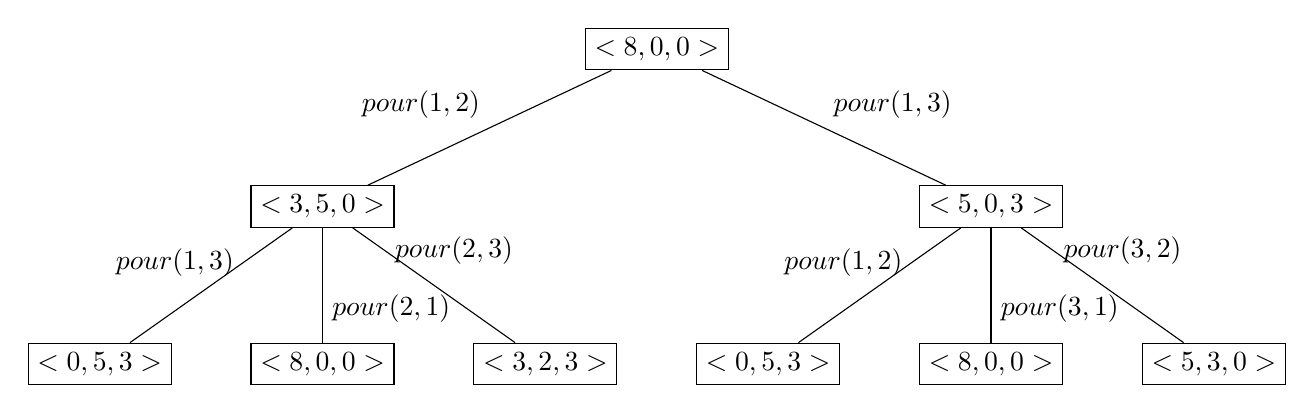
\begin{tikzpicture}[every tree node/.style={draw},
   level distance=2cm,sibling distance=1cm,
   edge from parent path={(\tikzparentnode) -- (\tikzchildnode)}]
\Tree
[.{$<8, 0, 0>$}
    \edge node[auto=right] {$pour(1, 2)$};
    [.{$<3, 5, 0>$}
       \edge node[left,pos=.3] {$pour(1, 3)$};
       {$<0, 5, 3>$}
       \edge node[right,pos=.7] {$pour(2, 1)$};
       {$<8, 0, 0>$}
       \edge node[right,pos=.2] {$pour(2, 3)$};
       {$<3, 2, 3>$}
    ]
    \edge node[auto=left] {$pour(1, 3)$};
    [.{$<5, 0, 3>$}
        \edge node[left,pos=.3] {$pour(1, 2)$};
        {$<0, 5, 3>$}
        \edge node[right,pos=.7] {$pour(3, 1)$};
        {$<8, 0, 0>$}
        \edge node[right,pos=.2] {$pour(3, 2)$};
        {$<5, 3, 0>$}
    ]
]
\end{tikzpicture}

Discuss the implications of this child node expansion order for Depth-First Search.

\begin{solution}[5in]
In basic Depth-First Search without repeated state-avoidance, the algorithm will get stuck decending an infinite path down the left side of the search tree, as shown in the first four levels of the search tree.

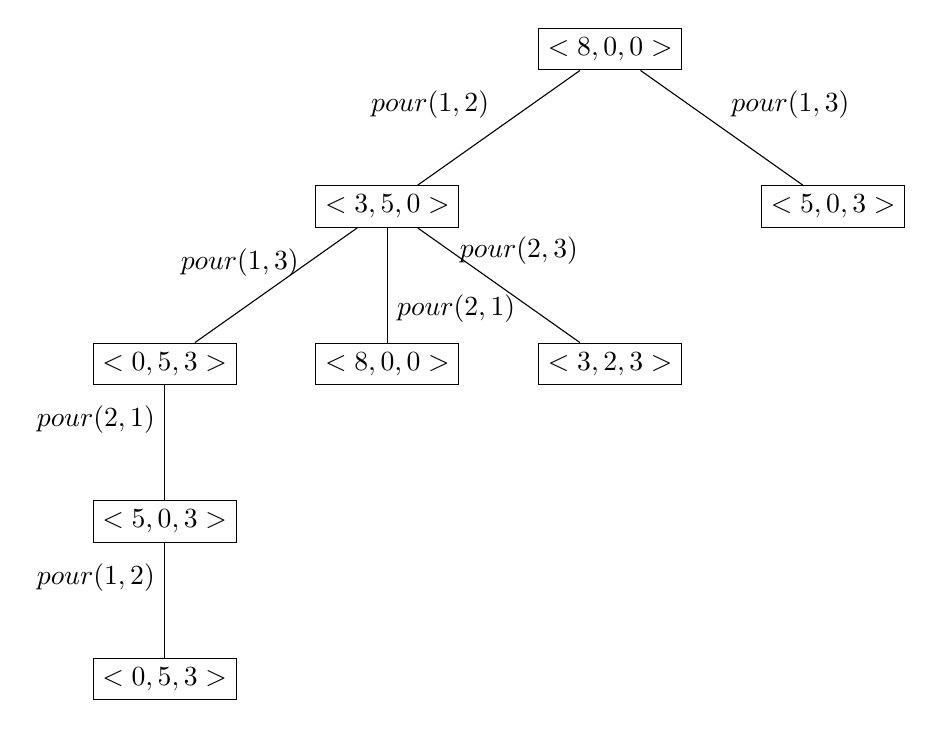
\begin{tikzpicture}[every tree node/.style={draw},
   level distance=2cm,sibling distance=1cm,
   edge from parent path={(\tikzparentnode) -- (\tikzchildnode)}]
\Tree
[.{$<8, 0, 0>$}
    \edge node[auto=right] {$pour(1, 2)$};
    [.{$<3, 5, 0>$}
       \edge node[left,pos=.3] {$pour(1, 3)$};
       [.{$<0, 5, 3>$}
         \edge node[left,pos=.3] {$pour(2, 1)$};
         [.{$<5, 0, 3>$}
           \edge node[left,pos=.3] {$pour(1, 2)$};
           {$<0, 5, 3>$}
         ]
       ]
       \edge node[right,pos=.7] {$pour(2, 1)$};
       {$<8, 0, 0>$}
       \edge node[right,pos=.2] {$pour(2, 3)$};
       {$<3, 2, 3>$}
    ]
    \edge node[auto=left] {$pour(1, 3)$};
    {$<5, 0, 3>$}
]
\end{tikzpicture}

\end{solution}

\question Is Breadth-First Search subject to the same problems discussed in the previous question?  Why, or why not?

\begin{solution}[1in]
No, because Breadth-First Search expands all the nodes at a particular level in the search tree before moving to the next level.
\end{solution}

\newpage

\question Is Breadth-First Search complete?  Why, or why not?

\begin{solution}[1in]
Yes, because it exands all nodes at each level successively, guaranteeing it will not miss a goal state as the depth of the search tree increases.
\end{solution}

\question Is Depth-First Search complete?  Why, or why not?

\begin{solution}[1in]
No, because even if cycles are avoided, DFS could get stuck searching an infinite in inifinite state spaces.
\end{solution}

\question What is the simplest way to modify Depth-First Search so that it does not descend an infinite path?

\begin{solution}[1.25in]
Depth-Limited Depth-First Search limits the depth to which Depth-First Search expands nodes.  This modification can lead to a complete expansion of the tree to the specified depth-limit.
\end{solution}

\question Discuss the most important implication of modifying Depth-First Search so that it does not descend an infinite path.

\begin{solution}[1.25in]
If there is no goal state within the depth limit for Depth-Limited Depth-First Search, then the algorithm will not find a goal state.
\end{solution}

\question Describe an algorithm that uses Depth-First Search but is complete.

\begin{solution}[1.75in]
Iterative-Deepening Depth-First Search simply runs Depth-Limited Depth-First Search for iteratively increasing depth limits until a goal state is found.
\end{solution}

\question What is the primary tradeoff between Bread-First Search and Depth-First Search?

\begin{solution}[1in]
Depth-First Search uses less memory, $O(bm)$ where $b$ is branching factor and $m$ is max depth of tree vs Breadth-First Seaarch, which uses $O(b^d)$ memory because it stores all the nodes in each level as it expands the search tree.
\end{solution}

\end{questions}

\end{document}
